%basic_buried_waveguide
\begin{figure}[!ht]
\centering
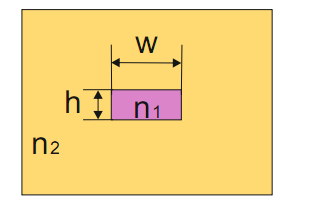
\includegraphics[width=0.6\textwidth]{bilder/buried_waveguide}
\caption{Schema of a basic buried waveguide.}
\label{fig:buried_waveguide}
\end{figure}
In agreement with the waveguide in the experiment, the buried waveguide model like Fig. \ref{fig:buried_waveguide} in this section obtains the identical dimensions ($w01\mu$m and $h00.5\mu$m) and refractive indexes (n$_{1}$ and n$_{2}$) with the original waveguide.\\ 
Fig. \ref{fig:curve_coupling_basic_buried_waveguide} shows the coupling efficiency between TLF and the regular buried waveguide due to the frequencies. The coupling efficiency at the working frequency $282$THz reaches about $51.3\%$, which is relative higher than that of the stripped rib waveguide. This value will be referred for further discussion about coupling from TLF to the lensed waveguide.  
\begin{figure}[!ht]
\centering
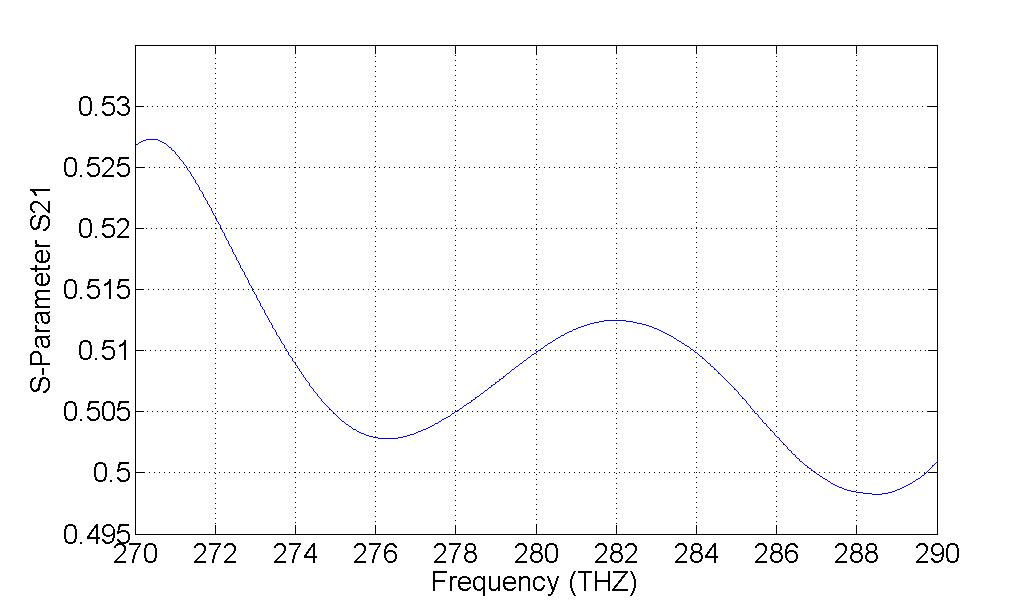
\includegraphics[width=0.8\textwidth]{bilder/s21_sym_waveguide}
\caption{Coupling efficiency curve between TLF and the basic buried waveguide due to frequency domain.}
\label{fig:curve_coupling_basic_buried_waveguide}
\end{figure}
